\section{Arquitetura}\label{arquitetura}

Esta seção apresenta a arquitetura do barramento (intitulado ErlangMS) que está 
sendo proposto para apoiar as atividades de modernização 
de software do CPD. 

O ErlangMS é um barramento orientado a serviço (\textit{Enterprise Service Bus}, ESB) 
que est\'{a} sendo desenvolvido na linguagem Erlang. O barramento 
fornece a camada de serviço para a abordagem SOA proposta neste trabalho. De acordo 
com \cite{SOAPractice:2007}, um ESB possibilita o uso de serviços, unificando o acesso a esses serviços através de uma camada intermediadora entre componentes de software (denominados serviços) e as aplicações 
que consomem estes serviços.

Nesse sentido, ErlangMS foi idealizado para servir de elo entre os 
sistemas da Universidade e a camada de negócio (tipicamente 
implementada usando a linguagem Java). A implementa\c c\~{a}o 
de um novo barramento (em vez da ado\c c\~{a}o de um barramento existente), 
possibilitou uma melhor compreens\~{a}o do estilo arquitetural REST e o dom\'{i}nio de alguns 
elementos chave propostos no ErlangMS, como a estrutura de eventos e os recursos de toler\^{a}ncia 
a falha.

Na arquitetura proposta, o esquema de comunicação do barramento com os demais sistemas 
ocorre por meio de 
duas vias distintas. Na primeira via, existe a comunicação do cliente para 
invocar algum serviço no barramento. Essa comunicação ocorre por meio de uma 
interface REST, razão pela qual o cliente (que pode ser qualquer sistema, 
independente da sua linguagem de programação ou plataforma) 
precisa suportar chamadas de serviços em REST (tipicamente requisições HTTP). 
Na segunda via existe a comunicação 
do barramento com os módulos de negócio. Essa comunicação acontece através do sistema de mensageria 
disponível em Erlang, que possui recursos para comunicação assíncrona 
com várias linguagens de programação.

Com essa estratégia, a linguagem Java continua sendo utilizada para 
escrever os módulos de negócio, uma linguagem apropriada para esse 
tipo de tarefa e de relativo domínio pelo CPD. O barramento fica responsável pela 
comunicação e gerenciamento de eventos, a escalabilidade, o monitoramento 
e o gerenciamento do catálogo de serviços. 
É importante destacar que essa arquitetura dá ênfase para um modelo de 
computação assíncrona, onde os sistemas não precisam ficar aguardando 
solicitações de serviço que podem ser demoradas. 

A decisão da linguagem Erlang, na implementação do barramento, 
deu-se porque ela possui um ambiente de execução e um modelo de concorrência 
baseado em troca de mensagens entre atores, integrados na própria linguagem, o que facilitam 
a construção de sistemas distribuídos escaláveis e tolerante a falhas.
Espera-se com essa abordagem, que os sistemas novos e os legados possam coexistir, 
enquanto a modernização estiver sendo executada, com ambos acessando a mesma lógica de negócio. 


\subsection{Requisitos da Arquitetura}

O barramento foi projetado para ser aderente a arquitetura REST e utilizar o formato JSON (restrição técnica adotada visando facilitar a implementação) para a troca de mensagens com o cliente. No lado da comunicação do barramento com a camada de negócio, a tecnologia empregada será \texttt{jInterface}, um módulo para comunicação com processos Java disponível em Erlang.

\subsection{Catálogo de Serviços}

Um componente chave dessa arquitetura é o conceito de 
catálogo de serviços, que em linhas gerais, dá visibilidade aos serviços 
disponibilizados, permitindo a reusabilidade dos componentes de software, 
uma vez que, estando o serviço publicado no barramento de serviços (conforme 
visto na Figura \ref{fig:catalogo}), poderá ser acessado por diversas outras aplicações, inclusive aquelas que não estavam previstas inicialmente.


\begin{figure}[htb]
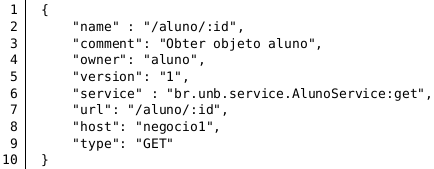
\includegraphics[scale=0.6]{figuras/catalogo.png}
\caption{Exemplo de catálogo de serviço para descrever o recurso aluno}
\label{fig:catalogo}
\end{figure}

O catálogo de serviço está sendo concebido para ser administrado a partir 
de um arquivo em formato JSON. Este arquivo deverá conter a descrição dos 
metadados que descrevem os serviços oferecidos pelo barramento. 
As informações contidas nesse catálogo seguem o modelo descrito 
por \cite{OASISRefArch:2012}. Entre as informações disponíveis estão 
o nome e a descrição do serviço, o responsável pelo serviço, a URL, 
os parâmetros do serviço, se o serviço é assíncrono ou não, entre outros dados.

Alguns requisitos técnicos para a arquitetura foram estipulados, como descritos a seguir:

\begin{enumerate}[(RQ1)]

\item Prover uma interface REST para comunicação com os clientes, por meio de uma API REST, suportando o subconjunto de operações HTTP \textit{GET, POST, PUT e DELETE}. 
O objetivo \'{e} fornecer uma tecnologia agnóstica sobre a linguagem de programa\c c\~{a}o
para troca de mensagens. Cada requisição deverá conter toda informação do 
pedido e nenhum estado das comunicações entre as mensagens deverá ser mantido. 
Além disso, cada recurso será unicamente direcionado através da sua URI.

\item Escalabilidade e tolerância a falhas (Requisito não funcional). Deve suportar 
duas características de qualidade de serviço (QoS): a escalabilidade 
(suportar uma carga de trabalho maior quando necessário) e tolerância a falhas 
(recuperar-se de possíveis falhas no processamento das solicitações). Além disso, 
uma requisição a um serviço de longa duração não deve comprometer o processamento 
das demais solicitações e qualquer falha no atendimento deverá retornar ao cliente 
na forma de uma mensagem JSON descrevendo o motivo do erro.

\item Monitoramento e Gerenciamento do Barramento. O barramento deverá prover um portal de gerenciamento, onde será possível monitorar o consumo dos serviços e listar 
os serviços disponíveis no catálogo.

\end{enumerate}


\subsection{Implementação do Barramento}

As características do projeto inicial foram trabalhadas na disciplina de \textit{Construção de Software} (CS). No primeiro seminário da disciplina, apresentou-se o protótipo da arquitetura do módulo HTTP (para suportar a interface de comunicação REST). Entre os desafios, destacam-se o parser do cabeçalho e a leitura completa do \textit{payload} da requisição HTTP.

Com a implementação do módulo HTTP, o próximo 
passo foi desenvolver o módulo de roteamento das requisições. Como não existia ainda um catálogo de serviço implementado, as rotas dos serviços 
foram inseridas diretamente no código fonte. Dois módulos de serviços foram criados 
para testar o roteamento preliminar: o serviço que trata a URL ‘‘/‘‘ e responde com a 
mensagem \{‘‘\textit{message}‘‘: ‘‘\textit{It works}‘‘\} e o serviço que trata 
a URL ‘‘/\textit{hello}\_\textit{world}‘‘ e retorna a 
mensagem \{‘‘\textit{message}‘‘: ‘‘Ola mundo‘‘\}.

Posteriormente, com a arquitetura básica pronta, o código foi refatorado com os princípios de design da \textit{Open Telecom Plataform} (OTP), 
o \textit{framework} da linguagem Erlang para construção de aplicações escaláveis e tolerante a falhas. Foram implementados o catálogo de serviços (a partir da leitura de um arquivo JSON), desenvolvido o módulo \textit{dispatcher} para localizar os serviços nesse catálogo (a partir da URL e do método HTTP da requisição) e redirecionar para o serviço correspondente. Também foi adicionado suporte para a transformação 
dos dados de/para JSON (de forma transparente dos processos de serviços) e 
implementado o tratamento de erros HTTP para os códigos de retorno mais comuns.

O próximo passo no desenvolvimento foi adicionar os recursos de supervisão da OTP 
(processos que supervisionam outros processos filhos) para gerar a árvore de supervisão 
e permitir ao barramento recuperar-se de possíveis falhas.

Para garantir a qualidade desejada, 62 testes automatizados foram gerados com a biblioteca Eunit (módulo para testes unitários do Erlang) para testar o funcionamento dos módulos implementados e simular requisições HTTP/REST (como um cliente faria) ao barramento de modo a analisar o comportamento do barramento durante sua execução.

As próximas versões do barramento vão focar na parte da integração dos processos em Java, utilizando a biblioteca \textit{jInterface} do Erlang. O desenvolvimento desta etapa será realizado em conjunto com a próxima etapa do trabalho, ou seja, durante o estudo de caso que será apresentado na próxima seção.

